\documentclass[aspectratio=169,t,9pt]{beamer}
\usepackage[utf8]{inputenc}
\usepackage{xcolor}
\usepackage{graphicx}
\usepackage{tikz}
\usepackage{amsmath}
\usepackage{amsfonts}
\usepackage{booktabs}

% Bitcoin orange color theme
\definecolor{bitcoinorange}{RGB}{247,147,26}
\definecolor{bitcoindark}{RGB}{33,33,33}
\definecolor{bitcoinlight}{RGB}{255,255,255}

% Metropolis theme - Modern, minimalist Beamer theme
% Source: https://github.com/matze/mtheme
% License: Creative Commons Attribution-ShareAlike 4.0 International
% Features: Clean design, optional progress bar, maximizes content space
\usetheme[progressbar=foot]{metropolis}  % Enable progress bar in footer

% Customize colors for Bitcoin orange theme
\setbeamercolor{progress bar}{fg=bitcoinorange, bg=bitcoindark!50}  % Orange fill, subtle dark background for unfilled part
\setbeamercolor{palette primary}{bg=bitcoinorange,fg=white}
\setbeamercolor{palette secondary}{bg=bitcoindark,fg=white}
\setbeamercolor{structure}{fg=bitcoinorange}
\setbeamercolor{frametitle}{bg=bitcoinorange,fg=white}
\setbeamercolor{title}{bg=bitcoindark,fg=bitcoindark}  % Dark text for visibility on light background
\setbeamercolor{block title}{bg=bitcoinorange,fg=white}
\setbeamercolor{block body}{bg=bitcoinorange!10}
\setbeamercolor{frame footer}{bg=bitcoinorange!10}
\setbeamercolor{date in head/foot}{bg=bitcoinorange, fg=bitcoinlight}

% Adjust fonts
\setbeamerfont{footnote}{size=\tiny}

% Title information
\title[Bitcoin Missverständnisse]{\vspace{1.5in}Bitcoin: Häufige Missverständnisse und was wirklich dahinter steckt}
\subtitle{Ein faktenbasierter Impulsvortrag}
\author{Bitcoin Entdecken / Bitcoin Austria}
\date{\today}
\institute{}
\titlegraphic{\center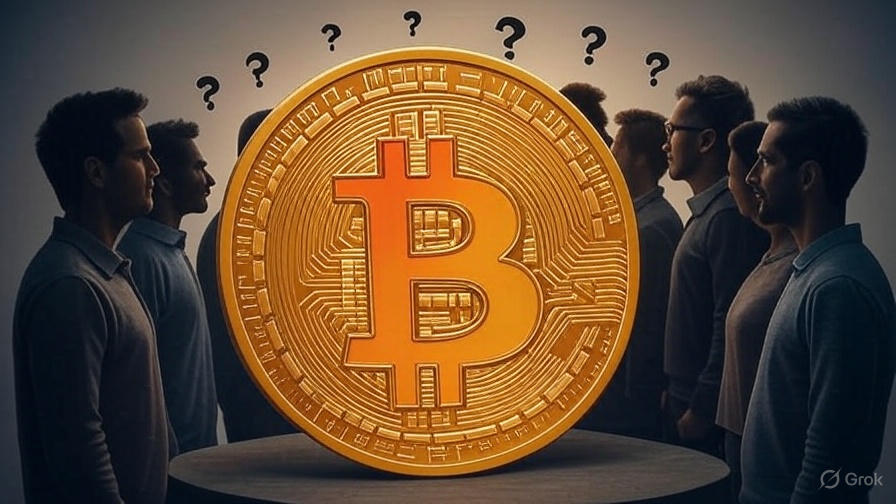
\includegraphics[width=0.4\textwidth,keepaspectratio]{pix/title-grafik.jpg}}

% Custom footer with frame numbers only
\setbeamertemplate{footline}{
    \leavevmode%
    \hbox{%
        \begin{beamercolorbox}[wd=\paperwidth,ht=2.25ex,dp=1ex,right]{date in head/foot}%
            \insertframenumber{} / \inserttotalframenumber\hspace*{2ex}
        \end{beamercolorbox}%
    }
    \vskip0pt%
}

% Counter for misconceptions
\newcounter{mvnum}
\setcounter{mvnum}{0}
% Include auto-generated count of misconceptions
% Auto-generated file - DO NOT EDIT MANUALLY
% Generated by count-misconceptions.sh on Do 31 Jul 2025 11:32:40 CEST
\newcommand{\totalmisconceptions}{11}


% Remove top margin from beamer frames
\setbeamersize{text margin left=10pt,text margin right=10pt}

% Custom frametitle with logo on the right - no top margin
\setbeamertemplate{frametitle}{
    \nointerlineskip%
    \begin{beamercolorbox}[wd=\paperwidth,ht=2.5ex,dp=1ex,leftskip=0pt,rightskip=0pt]{frametitle}
        \hbox to \paperwidth{%
            \begin{beamercolorbox}[wd=0.75\paperwidth,left]{frametitle}%
                \hspace*{1ex}\usebeamerfont{frametitle}\insertframetitle%
            \end{beamercolorbox}%
            \begin{beamercolorbox}[wd=0.25\paperwidth,right]{frametitle}%
                \hfill\raisebox{-0.5ex}{\includegraphics[height=3ex,keepaspectratio]{logo-bitcoin-entdecken.pdf}}\hspace*{1ex}%
            \end{beamercolorbox}%
        }
    \end{beamercolorbox}
}


% Macro for misconception slides with consistent layout
\newcommand{\misconceptionslide}[5][]{%
    % #1: Optional image path (if provided, image shows on first slide where facts appear later)
    % #2: Frame title (e.g., "Umweltauswirkungen")
    % #3: Misconception text (in quotes)
    % #4: Facts list items
    % #5: Fazit text
    \stepcounter{mvnum}
    \subsection{\arabic{mvnum}. #2}
    \begin{frame}<1-2>{M\arabic{mvnum}: #2}
        \begin{columns}[T]
            \begin{column}[T]{0.48\textwidth}
                \begin{block}{Das Missverständnis}
                    \vspace{0.5em}
                    \textit{``#3''}
                    \vspace{0.5em}
                \end{block}
            \end{column}
            \hspace{0.02\textwidth}
            \begin{column}[T]{0.48\textwidth}
                % Optional image only visible on first slide (where facts will appear later)
                \ifx\relax#1\relax
                    % No image provided
                \else
                    \only<1>{
                        \vspace{1em}
                        \centering
                        \includegraphics[width=0.95\textwidth,keepaspectratio]{#1}
                        \vspace{1em}
                    }
                \fi
                \onslide<2->{
                    \begin{block}{Die Fakten}
                        \vspace{0.3em}
                        \begin{itemize}
                            \setlength{\itemsep}{0.3em}
                            #4
                        \end{itemize}
                        \vspace{0.3em}
                    \end{block}
                }
            \end{column}
        \end{columns}
        
        \vfill
        
        \onslide<2->{
            \textcolor{bitcoinorange}{\textbf{Fazit:}} #5
        }
    \end{frame}
}

\begin{document}

% Title slide
\begin{frame}
    \titlepage
\end{frame}

% Table of contents
\begin{frame}{Überblick}
    \tableofcontents
\end{frame}

\begin{frame}{Warum entstehen Bitcoin-Missverständnisse?}
    \begin{itemize}
        \item \textbf{Komplexe Technologie} - Schwer verständlich für Laien
       \item \textbf{Falscher Fokus} - Die eigentlichen Fragen werden nicht gestellt
        \item \textbf{Medienverzerrung} - Sensationelle Berichterstattung
        \item \textbf{Schnelle Entwicklung} - Veraltete Informationen halten sich hartnäckig
        \item \textbf{Emotionale Diskussionen} - Fakten vs. Meinungen
        \item \textbf{Interessenskonflikte} - Verschiedene Akteure mit eigenen Agenden
    \end{itemize}
    \vspace{2em}
    \begin{alertblock}{\textcolor{white}{Ziel dieser Präsentation}}
        Fakten statt Mythen - Was steht hinter den Argumenten?
    \end{alertblock}
\end{frame}

\section{Die \totalmisconceptions\ häufigsten Missverständnisse}

\misconceptionslide{Umweltauswirkungen}{Bitcoin-Mining verbraucht zu viel Energie und zerstört die Umwelt}{%
        \item Nur 0,54\% des globalen Stromverbrauchs\footnotemark
        \item Energieverbrauch \textit{essentiell}, nicht ``sinnlos''.
        \item Über 50\% erneuerbare Energiequellen\footnotemark
        \item Überschussenergie aus alternativen Quellen, macht diese lukrativ
        \item Weniger umweltschädlich als Goldbergbau
        \item 87\% der Mining-Hardware wird recycelt\footnotemark
        \only<2->{\footnotetext[1]{Cambridge Centre for Alternative Finance}}
        \only<2->{\footnotetext[2]{Cambridge Digital Mining Industry Report 2025}}
        \only<2->{\footnotetext[3]{z.B. 21 Energy}}
    }{Mining-Effizienz steigt kontinuierlich, Umweltimpact nimmt ab.}

\misconceptionslide{Kein intrinsischer Wert}{Bitcoin hat keinen intrinsischen Wert, daher ist es wertlos}{%
        \item Bitcoin hat keinen laufenden Erträge, daher nicht vergleichbar
        \item Nutzen 1: technisch limitiert auf 21 Mio
        \item Nutzen 2: Zensurresistenz
        \item Nutzen 3: Globales Zahlungsnetzwerk
        \only<2->{\footnotetext[1]{Emily Stanhope und der Ökonom Charles Brandt, in ``Review of Economic Philosophy''}}
	}{Es gibt keinen intrinsischen Wert, sondern der Wert entsteht durch gesellschaftliche Zuschreibung und kollektive Akzeptanz\footnotemark}

\misconceptionslide{Volatilität}{Bitcoin ist zu volatil, um als Währung oder Wertaufbewahrung zu funktionieren}{%
        \item Volatilität nimmt langfristig ab, wenn auch weniger als gedacht
        \item Weniger volatil als 33 S\&P 500 Aktien
        \item Typisch für neue Asset-Klassen
        \item Institutionelle Adoption stabilisiert
    }{Reifung des Marktes führt zu weniger Volatilität.}

\misconceptionslide{Regulierung}{Bitcoin hat keine rechtliche Grundlage und wird verboten werden}{%
        \item Regulierungsrahmen entwickeln sich schnell
        \item USA und EU schaffen klare Gesetze
        \item EU: MiCA-Verordnung erlaubt Bitcoin \& Co.
        \item Institutionelle Compliance wächst
        \item Verbote schwer durchsetzbar
    }{Rechtliche Klarheit nimmt weltweit zu.}

\misconceptionslide[pix/bitcoin-skalieren.jpg]{Skalierbarkeit}{Bitcoin kann nur 3-4 Transaktionen pro Sekunde verarbeiten}{%
        \item Blockchain-Trilemma: Skalierbarkeit vs. Sicherheit vs. Dezentralisierung
        \item Lightning Network: bis zu 1 Million TPS möglich
        \item Visa: 65.000 TPS, 150 Mio. Transaktionen/Tag\footnotemark
        \item Bitcoin Transaktionsvolumen: 20 Bio. \$ vs. Visa 13 Bio. \$\footnotemark
	\only<2->{\footnotetext[1]{Visa Inc. Annual Report 2023}}
	\only<2->{\footnotetext[2]{Sygnum Bank Report, 2024}}
        \item Lightning theoretisch 15x schneller als Visa - global, ohne Intermediäre
    }{Bitcoin übertrifft Visa bereits im Transaktionsvolumen und bei Second-Layer-Geschwindigkeit.}

\misconceptionslide{Spekulationsblase}{Bitcoin ist eine Spekulationsblase}{%
 	\item Blasen sind kurzfristig, über Monate, nicht über 10 Jahre
        \item Wertspeicher für langfristiges Sparen
        \item Netzwerkeffekte schaffen Mehrwert
        \item Institutionelle Adoption validiert Use-Case
        \item Knappheit (21 Mio. Limit) ähnlich wie Gold
    }{Fundamentaler Nutzen wächst über reine Spekulation hinaus.}

\misconceptionslide[pix/bitcoin-schneeball.jpg]{Schneeballsystem}{Bitcoin ist ein Schneeballsystem}{%
        \item Schneeballsysteme versprechen fixe Auszahlungen durch neue Teilnehmer
        \item Bitcoin gibt keine Renditegarantien
        \item Keine zentrale Organisation oder strukturierte Vertriebsarchitektur
        \item Weltbank 2022: Bitcoin-Protokoll offen zugänglich und nicht verpflichtend\footnotemark
        \item Schweizer Finma stuft Bitcoin nicht als Schneeballsystem ein\footnotemark
\only<2->{\footnotetext[1]{World Bank Group, Distributed Ledger Technology and Digital Assets, 2022}}
\only<2->{\footnotetext[2]{FINMA Guidance 02/2019: Payments on the blockchain}}
    }{Bitcoin erfüllt keines der zentralen Merkmale eines Schneeballsystems.}

\misconceptionslide{Kriminalität}{Bitcoin wird hauptsächlich für illegale Aktivitäten verwendet}{%
        \item Weniger als 1\% aller Transaktionen sind illegal (2024)
        \item Anteil illegaler Bitcoin-Transaktionen nur noch 0,34\%\footnotemark
        \item Traditionell: 2\% - 5\% des globalen BIP fließen durch illegale Kanäle\footnotemark
\only<2->{\footnotetext[1]{Chainalysis 2024}}
\only<2->{\footnotetext[2]{United Nations Schätzung}}
        \item Blockchain ist transparent und nachverfolgbar
        \item Europol betrachtet vor allem Bargeld und das traditionelle Bankensystem als relevant für Geldwäsche
    }{Bitcoin ist schlechter für Kriminalität als traditionelle Methoden.}

\misconceptionslide{Praktische Adoption}{Bitcoin hat keine praktische Anwendung im Alltag}{%
        \item Legales Zahlungsmittel (El Salvador, CAR)
        \item Corporate Treasury Asset
        \item Bitcoin-besicherte Kredite
        \item Grenzüberschreitende Zahlungen
        \item Langfristiges Sparen und Pensionsvorsorge
    }{Praktische Anwendungen wachsen kontinuierlich. Tägliche Zahlungen sind weniger sinnvoll, da nach Greshams Gesetz\footnotemark\ das ``schlechtere Geld'' bevorzugt ausgegeben wird.}
        \only<2->{\footnotetext{Wikipedia: Greshamsches Gesetz}}

\misconceptionslide{Bedenken von Zentralbanken}{Bitcoin bedroht die Geldpolitik und wird von Regierungen verboten}{%
        \item Ergänzt traditionelle Finanzsysteme
        \item Regierungen entwickeln crypto-freundliche Gesetze
        \item Zentralbanken erforschen digitale Währungen
        \item Banken vergeben Bitcoin-backed Loans: ``Bitcoin-Kreditvergabe ist eine logische Erweiterung des Krypto-Dienstleistungsportfolios der Banken''\footnotemark
\only<2->{\footnotetext[1]{Sopra Banking Software, 2024}}
        \item Hedge gegen Geldpolitik-Versagen
    }{Koexistenz statt Konkurrenzkampf mit traditioneller Finanzwelt.}

\misconceptionslide{Technische Sicherheit}{Bitcoin kann gehackt werden}{%
        \item 99,98\% Uptime seit 2009
        \item Dezentralisierung verhindert Single Point of Failure
        \item Protokoll wird durch zehntausende Nodes robust abgesichert
        \item Kritische Netzwerk-Updates erfordern breiten Konsens\footnotemark
\only<2->{\footnotetext[1]{The Blocksize War: The battle over who controls Bitcoin's protocol rules, Jonathan Bier}}
    }{Bitcoin ist seit über 15 Jahren ohne erfolgreichen Hack im Betrieb.}

\begin{frame}{Was lernen wir daraus?}
    \begin{alertblock}{\textcolor{white}{Schlüsselerkenntnisse}}
        \begin{enumerate}
            \item Viele Kritikpunkte basieren auf \textbf{veralteten Informationen}
            \item Das technische Ökosystem hinter Bitcoin wächst \textbf{rasant}
            \item \textbf{Faktendaten} widersprechen oft den Mediennarrativen
            \item \textbf{Institutionelle Adoption} validiert Bitcoins Legitimität
            \item \textbf{Umweltauswirkungen} nehmen ab, während Nutzen steigt
            \item Bitcoin erfüllt bereits heute wichtige \textbf{Finanzfunktionen}
            \item \textbf{Regulatorische Klarheit} entsteht weltweit
        \end{enumerate}
    \end{alertblock}

    \vspace{0.5em}
    \begin{block}{Empfehlungen}
        \begin{itemize}
            \item \textbf{Informieren Sie sich aus seriösen und aktuellen Quellen!}
            \item Hinterfragen Sie emotionale Argumente und suchen Sie nach Fakten
            \item Verstehen Sie den Unterschied zwischen Bitcoin-Protokoll und Exchanges
            \item Berücksichtigen Sie die schnelle Entwicklung des Ökosystems
        \end{itemize}
    \end{block}
\end{frame}

\begin{frame}{Quellen und weitere Informationen}
    \footnotesize
    \begin{itemize}
        \item \href{https://www.jbs.cam.ac.uk/faculty-research/centres/alternative-finance/}{Cambridge Centre for Alternative Finance}
        \item \href{https://www.jbs.cam.ac.uk/wp-content/uploads/2025/04/2025-04-cambridge-digital-mining-industry-report.pdf}{Cambridge Digital Mining Industry Report 2025}
        \item \href{https://21energy.com/}{21 Energy}
        \item Emily Stanhope und der Ökonom Charles Brandt, in ``Review of Economic Philosophy'' (Academic citation - URL not publicly available)
        \item \href{https://s29.q4cdn.com/385744025/files/doc_downloads/2023/Visa-Inc-Fiscal-2023-Annual-Report.pdf}{Visa Inc. Annual Report 2023}
        \item \href{https://www.sygnum.com/wp-content/uploads/2024/11/Sygnum-Future-Finance-Report-2024-institutional-crypto-market_download.pdf}{Sygnum Bank Future Finance Report 2024}
        \item World Bank Group, Distributed Ledger Technology and Digital Assets, 2022 (Specific document not found online)
        \item \href{https://www.finma.ch/~/media/finma/dokumente/dokumentencenter/myfinma/4dokumentation/finma-aufsichtsmitteilungen/20190826-finma-aufsichtsmitteilung-02-2019.pdf?sc_lang=en}{FINMA Guidance 02/2019: Payments on the blockchain}
        \item \href{https://go.chainalysis.com/crypto-crime-2024.html}{Chainalysis 2024 Crypto Crime Report}
        \item \href{https://www.unodc.org/documents/data-and-analysis/Studies/Illicit_financial_flows_2011_web.pdf}{United Nations Office on Drugs and Crime: Illicit Financial Flows Study}
        \item Sopra Banking Software, 2024 (Specific publication not found online)
        \item \href{https://www.amazon.com/Blocksize-War-controls-Bitcoins-protocol/dp/B08YQMC2WM}{The Blocksize War: The battle over who controls Bitcoins protocol rules} - Jonathan Bier
        \item \href{https://de.wikipedia.org/wiki/Greshamsches_Gesetz}{Wikipedia: Greshamsches Gesetz}
    \end{itemize}

    \vspace{1em}
    \begin{center}
        \textcolor{bitcoinorange}{\Large Fragen und Diskussion?}
        \\[1em]
        \textcolor{bitcoinorange}{\rule{0.5\textwidth}{2pt}}
    \end{center}
\end{frame}

\end{document}
